
%sudo apt-get install texlive-bibtex-extra
\documentclass{article}\usepackage[]{graphicx}\usepackage[]{color}
%% maxwidth is the original width if it is less than linewidth
%% otherwise use linewidth (to make sure the graphics do not exceed the margin)
\makeatletter
\def\maxwidth{ %
  \ifdim\Gin@nat@width>\linewidth
    \linewidth
  \else
    \Gin@nat@width
  \fi
}
\makeatother

\usepackage{Sweave}


\usepackage{float}
\usepackage{wrapfig}
\usepackage{hyperref}
\usepackage{booktabs}
\usepackage{longtable}
\usepackage[backend=bibtex, style=nature, citestyle=authoryear]{biblatex}
\usepackage[table]{xcolor}
\bibliography{WBVFM_IntroPar}
\newenvironment{knitrout}{}{}  %just a dummy environment
\makeatletter
\newcommand\gobblepars{%
    \@ifnextchar\par%
        {\expandafter\gobblepars\@gobble}%
        {}}
\makeatother
\title{Descriptives: SEA and MacArthur}
\IfFileExists{upquote.sty}{\usepackage{upquote}}{}
\begin{document}
\begin{knitrout}

\maketitle
\tableofcontents











\newpage
\section{Data}
% latex table generated in R 3.2.3 by xtable 1.8-2 package
% Tue Feb 16 11:04:46 2016
\begin{table}[ht]
\centering
\begingroup\footnotesize
\begin{tabular}{ll}
  \hline
Short Name & Long Name \\ 
  \hline
dari & dist\_to\_all\_rivers \\ 
  tc00 & hansen200\_tree\_cover \\ 
  dbri & dist\_to\_big\_rivers \\ 
  droa & dist\_to\_roads \\ 
  selv & srtm\_elevation \\ 
  sslp & srtm\_slope \\ 
  am50 & accessibility\_map \\ 
  gpw3 & gpw\_v3 \\ 
  nm6k & ndvi\_max\_mask\_lt6k \\ 
  lnye & ltdr\_yearly\_ndvi\_mean \\ 
  lnyx & ltdr\_yearly\_ndvi\_max \\ 
  alp4 & v4avg\_lights\_x\_pct \\ 
  nlc4 & v4composites \\ 
  ncc4 & v4composites\_calibrated \\ 
  at41 & terrestrial\_air\_temperature\_v4.01 \\ 
  pc41 & terrestrial\_precipitation\_v4.01 \\ 
   \hline
\end{tabular}
\endgroup
\caption{Variables used in this analysis.} 
\label{Variable_Table}
\end{table}

Variable names are defined in Table \ref{Variable_Table}.  

\newpage

\section{Descriptives}

%Cell-level statistics

% Table created by stargazer v.5.2 by Marek Hlavac, Harvard University. E-mail: hlavac at fas.harvard.edu
% Date and time: Tue, Feb 16, 2016 - 11:04:46 AM
\begin{table}[!htbp] \centering 
  \caption{Cell level descriptive statistics (N=6188)} 
  \label{} 
\begin{tabular}{@{\extracolsep{5pt}}lccccc} 
\\[-1.8ex]\hline 
\hline \\[-1.8ex] 
Statistic & \multicolumn{1}{c}{N} & \multicolumn{1}{c}{Mean} & \multicolumn{1}{c}{St. Dev.} & \multicolumn{1}{c}{Min} & \multicolumn{1}{c}{Max} \\ 
\hline \\[-1.8ex] 
tc00\_e & 6,188 & 39.216 & 33.918 & 0.000 & 97.590 \\ 
per\_loss\_e & 6,188 & 9.439 & 17.065 & 0.000 & 97.870 \\ 
dari\_e & 6,129 & 2,164.268 & 1,515.136 & 137.573 & 11,064.130 \\ 
droa\_e & 6,131 & 25,433.280 & 223,696.500 & 255.029 & 4,460,040.000 \\ 
selv\_e & 6,184 & 125.572 & 173.278 & 0.000 & 1,313.829 \\ 
sslp\_e & 6,184 & 1.373 & 2.148 & 0.000 & 17.241 \\ 
am50\_e & 6,181 & 385.607 & 286.001 & 4.342 & 1,828.021 \\ 
gpw3\_1990e & 6,156 & 79.584 & 1,312.301 & 0.100 & 90,440.270 \\ 
gpw3\_1995e & 6,156 & 93.991 & 1,552.600 & 0.119 & 107,002.400 \\ 
gpw3\_2000e & 6,156 & 107.989 & 1,785.916 & 0.137 & 123,083.300 \\ 
lnyx\_mean & 6,188 & 6,976.404 & 813.780 & 1,686.406 & 8,880.642 \\ 
ncc4\_mean & 6,188 & 0.144 & 1.317 & 0.000 & 56.921 \\ 
at41\_mean & 6,188 & 23.624 & 1.283 & 18.130 & 26.440 \\ 
pc41\_mean & 6,188 & 129.491 & 31.102 & 106.203 & 285.172 \\ 
\hline \\[-1.8ex] 
\multicolumn{6}{l}{Variables with 'mean' appendix are summaries of the yearly mean values.} \\ 
\end{tabular} 
\end{table} 


%ADM2-level statistics

% Table created by stargazer v.5.2 by Marek Hlavac, Harvard University. E-mail: hlavac at fas.harvard.edu
% Date and time: Tue, Feb 16, 2016 - 11:04:47 AM
\begin{table}[!htbp] \centering 
  \caption{ADM2 level descriptive statistics (N=176)} 
  \label{} 
\begin{tabular}{@{\extracolsep{5pt}}lccccc} 
\\[-1.8ex]\hline 
\hline \\[-1.8ex] 
Statistic & \multicolumn{1}{c}{N} & \multicolumn{1}{c}{Mean} & \multicolumn{1}{c}{St. Dev.} & \multicolumn{1}{c}{Min} & \multicolumn{1}{c}{Max} \\ 
\hline \\[-1.8ex] 
tc00\_e & 176 & 24.160 & 25.398 & 0.000 & 93.291 \\ 
per\_loss\_e & 176 & 7.046 & 10.188 & 0.000 & 51.251 \\ 
dari\_e & 175 & 2,167.215 & 754.885 & 665.675 & 5,706.997 \\ 
droa\_e & 176 & 36,945.490 & 172,528.300 & 1,227.143 & 1,777,850.000 \\ 
selv\_e & 176 & 76.027 & 112.420 & 3.331 & 694.954 \\ 
sslp\_e & 176 & 0.900 & 1.230 & 0.062 & 6.133 \\ 
am50\_e & 176 & 274.112 & 180.083 & 21.460 & 869.140 \\ 
gpw3\_1990e & 176 & 157.126 & 369.933 & 1.151 & 3,754.542 \\ 
gpw3\_1995e & 176 & 185.625 & 437.672 & 1.361 & 4,442.101 \\ 
gpw3\_2000e & 176 & 213.272 & 503.438 & 1.566 & 5,109.679 \\ 
lnyx\_mean & 176 & 6,557.321 & 780.621 & 4,459.846 & 8,207.006 \\ 
ncc4\_mean & 176 & 0.490 & 2.186 & 0.000 & 24.470 \\ 
at41\_mean & 176 & 23.902 & 1.142 & 20.912 & 26.440 \\ 
pc41\_mean & 176 & 122.580 & 26.040 & 106.203 & 285.172 \\ 
\hline \\[-1.8ex] 
\multicolumn{6}{l}{Variables with 'mean' appendix are summaries of the yearly mean values.} \\ 
\multicolumn{6}{l}{All variables represent the mean cell value within a ADM 2.} \\ 
\end{tabular} 
\end{table} 


\section{Forest Thresholds}
Because the Hansen dataset begins in the year 2000, it is not possible to conduct long-term analyses using this dataset alone.  
To mitigate this, we select to leverage the longer-term record (1982 to present) offered by the NASA Long Term Data Record (LTDR).
However, the LTDR has both a coarser resolution (5km, as opposed to 30 meters) as well as a different unit of measurement (Normalized Difference Vegetation Index) than the Hansen product.
To take advantage of the information in Hansen, as well as the long term record provided by the LTDR, we fuse the two data products together using the single year of forest cover data provided by Hansen (2000).
\par
The fusion process aggregates the Hansen 2000 30 meter cells to calculate a mean \% of forest cover estimated by Hansen within each 5km LTDR cell.  
We then contrast the mean annual values of NDVI present in LTDR to the forest cover values in Hansen, selecting only LTDR cells which have at least 10\% forest cover according to the Hansen dataset. 
\begin{figure}[H]
\caption{Relationship between LTDR 2000 NDVI and Hansen \% Forest Cover 2000, of LTDR cells with at least 10\% forest cover according to Hansen 2000.}
\label{LTDR_Hansen}
\centering
\begin{Schunk}

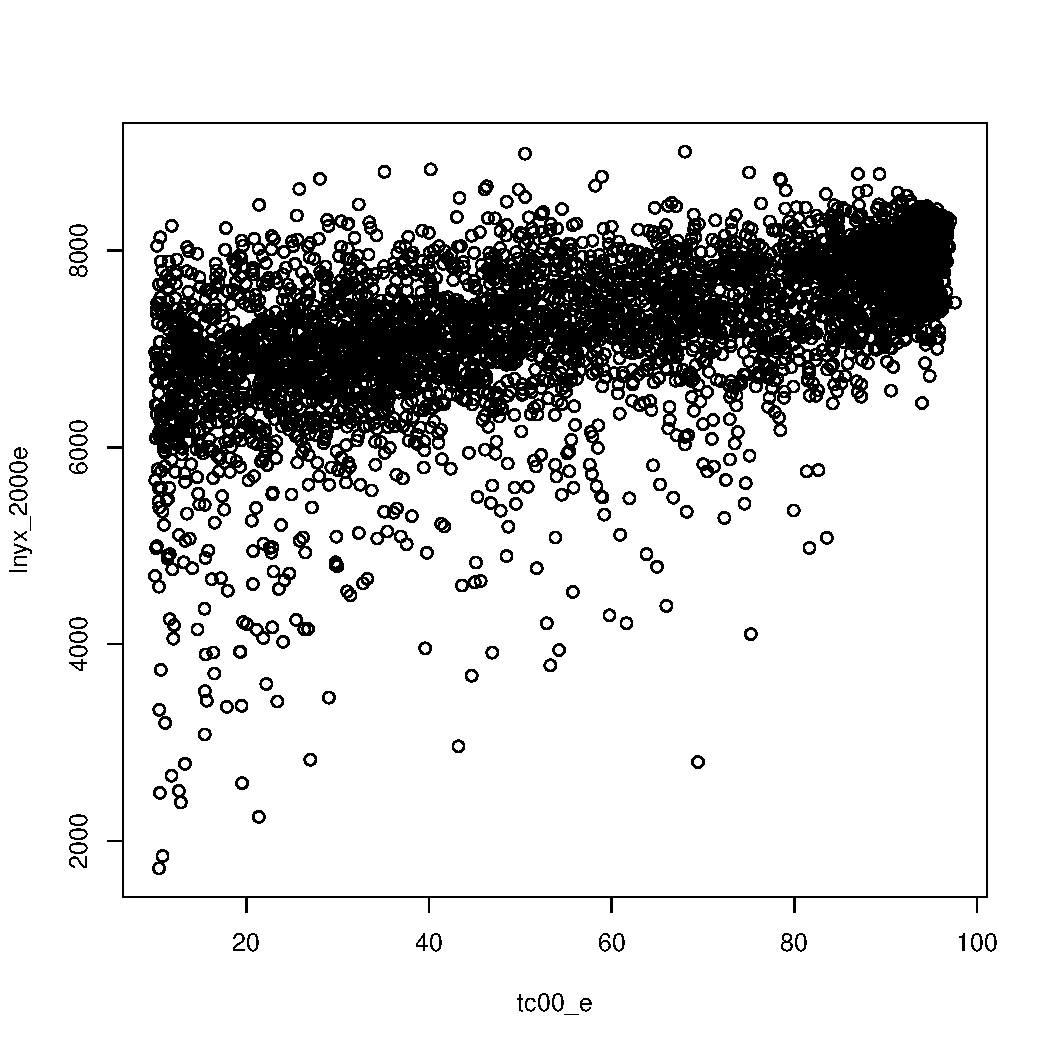
\includegraphics[width=0.8\linewidth]{figure/LTDR_NDVI-1} \end{Schunk}
\end{figure}
The distribution of NDVI values for the remaining LTDR cells can be seen in figure \ref{LTDR_Hansen}.  
As expected, we see a strong correlation - areas with higher levels of NDVI also tend to have higher levels of forest cover as estimated by Hansen.  
Because LTDR and Hansen are not independent products (Hansen leverages the same input as LTDR in the product production), this analysis does not suggest that one product can be used to independently verify the other.  
Rather, here we illustrate that backcasting forest cover using LTDR can serve as a proxy to produce a longer time series of information roughly analogous to the higher-resolution approach to detecting forest cover Hansen employs.
\begin{figure}[H]
\caption{Histogram of LTDR NDVI Values in (a) locations with >10\% forest cover in Hansen 2000, and (b) locations with <10\% forest cover in Hansen 2000.}
\label{NDVI_Hansen_hist}
\centering
\begin{Schunk}

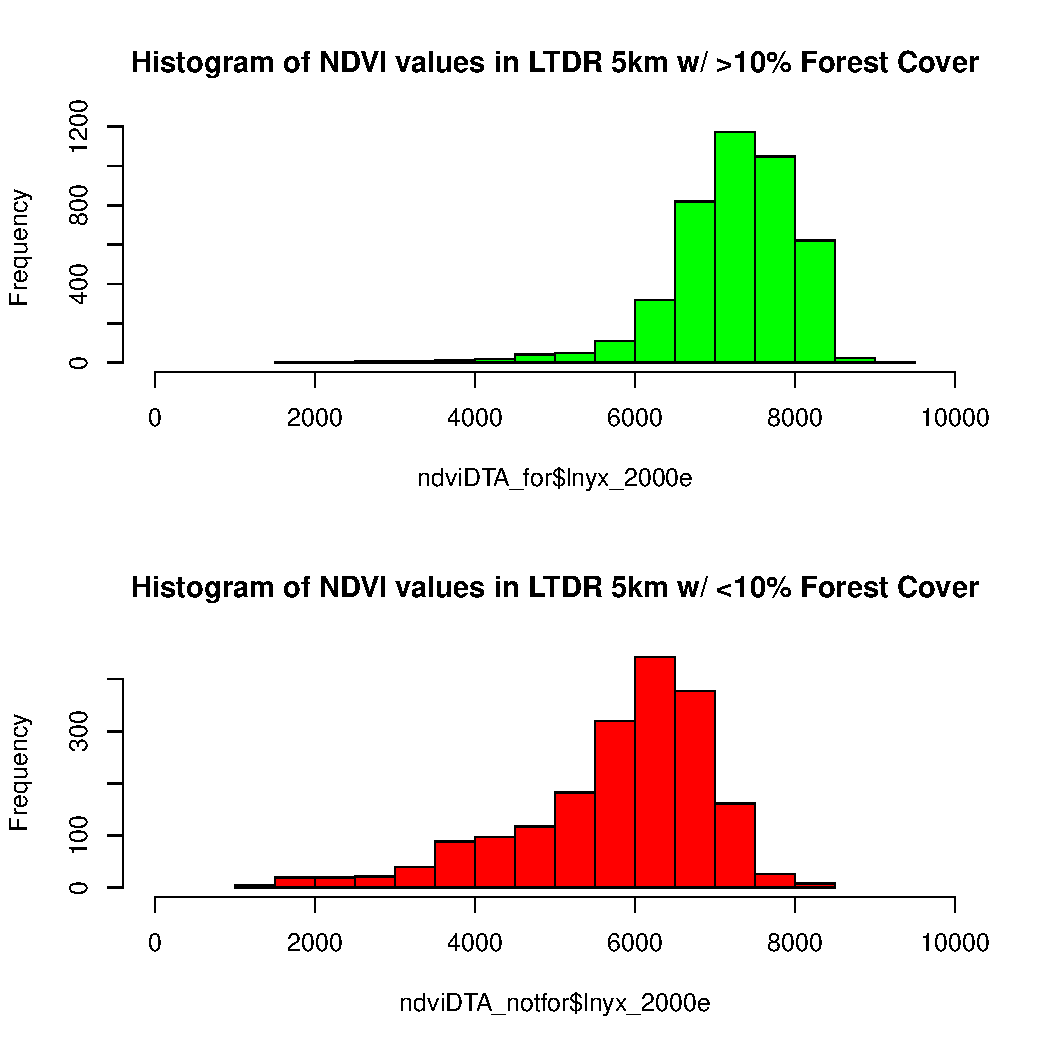
\includegraphics[width=0.8\linewidth]{figure/LTDR_NDVI_hist-1} \end{Schunk}
\end{figure}
\par
Using this information, for any historic or future LTDR (5km) unit of observation, the probability each unit is forest or non-forest is calculated based on a maximum likelihood decision rule.
The probability of each unit containing a forest is calculated, and all units which have a higher probability of inclusion into the "forest" class than "non-forest" class are used in later steps of the analysis.
The estimated probability density function to estimate inclusion into the forested class is calculated using the following equation:
\begin{equation}
\rho (x | c_{i}) = \frac{1}{(2\pi)^{1/2}*\sigma_{i}} * exp(-\frac{1}{2}*\frac{(x-\mu_{i})^{2}}{\sigma_{i}^{2}})
\end{equation}
where \textit{x} is the LTDR value of the unit being classified as forest or non-forest (represented as classes \textit{c}), \begin{math}\mu_{i}\end{math} is the estimated mean of all LTDR values determined to be included in class \textit{i} and \begin{math}\sigma_{i}^{2}\end{math} is the estimated variance of each class, i.e. \begin{math}x \in forest (c_{1}) \end{math}when:
\begin{equation}
\rho (x | c_{1}) * \rho(c_{1}) \geq \rho (x | c_{0}) * \rho(c_{0})
\end{equation}
where prior probabilities \begin{math} \rho(c_{i})\end{math} are established based on the probability of a LTDR pixel being classified as forest or non-forest in the year 2000 (i.e., the percent of the landscape occupied by each class).
\par


\end{knitrout}
\end{document}
